\title{MAT327 C\'alculo Num\'erico}
\author{Manuel Loaiza Vasquez}
\date{Noviembre 2021}

\begin{document}

\maketitle

\vspace*{-0.25in}
\centerline{Pontificia Universidad Cat\'olica del Per\'u}
\centerline{Lima, Per\'u}
\centerline{\mailto{manuel.loaiza@pucp.edu.pe}}
\vspace*{0.15in}

\begin{framed}
  Solucionario de la tercera pr\'actica. Instructor: Rub\'en Agapito.
\end{framed}

\begin{statement}{1}
  Use a plot to approximately locate all the roots of
  $f(x) = x^{-2} - \sin(x)$
  in the interval $[1/2, 4 \pi]$.
  Then find a pair of initial points for each root such that
  \[
    q(x) = f(x_k) + \frac{f(x_k) - f(x_{k - 1})}{x_k - x_{k - 1}} (x - x_k).
  \]
  converges to that root.
\end{statement}

\begin{solution}
  We want to find roots of the function $f$
  \begin{figure}[H]
    \centering
    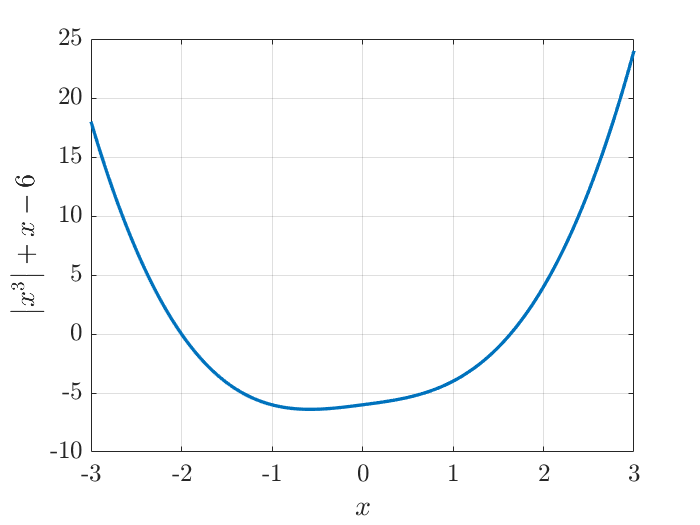
\includegraphics[scale=0.45]{graphics/plot-01.png}
    \caption{Plot of $f$ in $[1/2, 4 \pi]$}
  \end{figure}
  From the graph, it is clear that there are roots in the intervals
  $[0.8, 1.5], [2.5, 4], [5.5, 7]$ and $[9, 10]$.
  Using the secant method
  \lstinputlisting{scripts/algorithms/secant.m}
  the following code
  \lstinputlisting{scripts/problems/problem-01.m}
  outputs the approximated roots
  \verbatiminput{outputs/output-01.txt}
\end{solution}


\begin{statement}{2}
  Write a function that performs inverse quadratic interpolation for
  finding a root of $f$, give three initial estimates.
  To find the quadratic polynomial $q(y)$ passing through the three most recent points,
  use the built-in \texttt{polyfit} command.
  Test your function on the first problem from this section.
\end{statement}

\begin{solution}
  The following function performs inverse quadratic interpolation
  \lstinputlisting{scripts/algorithms/iqi.m}
  Examples 4.4.1 and 4.4.2 analyze the function $f(x) = x e^x - 2$
  and Example 4.4.3 the function $f(x) = x + \cos(10x)$ with real domain.
  We are going to test our function with these examples
  \lstinputlisting{scripts/problems/problem-02.m}
  obtaining the following roots:
  \verbatiminput{outputs/output-02.txt}
\end{solution}

\begin{statement}{3}
  Algoritmo de Romberg.
\end{statement}

\begin{statement}{a}
  Escriba una funci\'on en MATLAB que integre v\'ia el algoritmo de Romberg.
  Uno deber\'ia invocar la funci\'on como \texttt{R = romberg(f, a, b, n)},
  donde
  \texttt{f} es la funci\'on,
  \texttt{a} y \texttt{b} los extremos del intervalo
  y \texttt{n} el tama\~no de la tabla de Romberg.
  La funci\'on debe retornar como salida la tabla de Romberg completa.
  La mejor aproximaci\'on de la integral ser\'ia el valor en \texttt{R(n, n)}.
\end{statement}

\begin{solution}
  La siguiente funci\'on implementa el algoritmo de Romberg, donde
  $f$ es la funci\'on a integrar,
  $a$ y $b$ los extremos del intervalo de integraci\'on
  utilizando $2^n + 1$ puntos.
  \lstinputlisting{scripts/algorithms/romberg-algorithm.m}
\end{solution}

\begin{statement}{b}
  Use la funci\'on \texttt{romberg} para calcular las integrales
  \[
    \int_0^{\pi} \sin(x) \, dx \text{ y } \int_0^1 \sqrt{x} \, dx.
  \]
  Calcule tambi\'en los errores.
  Los valores exactos de las integrales son $2$ y $2 / 3$, respectivamente.
  Exhiba los errores a lo largo de la diagonal de la tabla
  y observe c\'omo cambia a lo largo de la diagonal.
\end{statement}

\begin{solution}
  Primero creamos la siguiente funci\'on para que imprima ambas tablas solicitadas
  \lstinputlisting{scripts/utils/print-tables.m}
  La funci\'on anterior llama a otras dos funciones.
  Una se encarga de imprimir los valores de la tabla de Romberg
  \lstinputlisting{scripts/utils/print-romberg.m}
  y la otra los errores absolutos de la tabla de Romberg con el valor exacto de la integral
  \lstinputlisting{scripts/utils/print-romberg-errors.m}
  Calculamos la primera integral
  \lstinputlisting{scripts/problems/problem-03-01.m}
  \verbatiminput{outputs/problem-03-01.txt}
  y la segunda
  \lstinputlisting{scripts/problems/problem-03-02.m}
  \verbatiminput{outputs/problem-03-02.txt}
  obteniendo como integrales num\'ericas $2$ y $0.665593$, respectivamente.
\end{solution}

\begin{statement}{c}
  Explique por qu\'e el algoritmo de Romberg
  nos da pobres resultados para la \'ultima integral.
  Use la funci\'on \texttt{integral} de MATLAB para calcular las integrales
  del \'item (b) usando $10^{-9}$ como tolerancia para ambas integraciones.
\end{statement}

\begin{solution}
  Localmente, he llamado a la funci\'on que calcula la segunda integral
  para valores de $n$ m\'as grandes, por ejemplo, $n = 12$, y usando seis
  d\'igitos de exactitud e igual seguimos teniendo un error absoluto distinto de cero
  \verbatiminput{outputs/output-03-03.txt}
  El algoritmo de Romberg nos da pobres resultados para esta \'ultima integral
  y necesitamos una cantidad bastante grande de puntos para mejorar el resultado
  puesto que la funci\'on $\sqrt{x}$ no tiene expansi\'on de Taylor alrededor de cero
  y debido a la extrapolaci\'on de Richardson, el error depender\'ia pr\'acticamente
  de su expansi\'on.

  Finalmente, usando el comando \texttt{integral} conseguimos
  \lstinputlisting{scripts/problems/problem-03-04.m}
  con integral num\'erica $2.000000000$ en la primera
  \lstinputlisting{scripts/problems/problem-03-05.m}
  y $0.666666667$ en la segunda.
\end{solution}


\begin{statement}{4}
  Considere la regla de cuadratura gaussiana con cuatro puntos en el intervalo $[-1, 1]$
  \[
    \int_{-1}^1 f(x) \, dx \approx a_1 f(x_1) + a_2 f(x_2) + a_3 f(x_3) + a_4 f(x_4)
  \]
  donde
  \begin{align*}
    x_1 &= -\sqrt{(3 - 4 \sqrt{0.3}) / 7}, \\
    x_2 &= -\sqrt{(3 + 4 \sqrt{0.3}) / 7}, \\
    x_3 &= \sqrt{(3 - 4 \sqrt{0.3}) / 7}, \\
    x_4 &= \sqrt{(3 + 4 \sqrt{0.3}) / 7}, \\
    a_1 = a_3 &= 1/2 + \sqrt{10 / 3} / 12, \\
    a_2 = a_4 &= 1/2 - \sqrt{10 / 3} / 12.
  \end{align*}
  Pruebe que la regla es exacta para todos los polinomios de grado menor o igual a siete.
\end{statement}

\begin{solution}
  Verifiquemos que la regla satisface la igualdad para $f(x) = 1, x, x^2$ y $x^3$.
  El caso $f(x) = 1$ es f\'acil de verificar
  \begin{align*}
    2 &= \left(\frac{1}{2} + \frac{1}{12}\sqrt{\frac{10}{3}}\right)
    + \left(\frac{1}{2} - \frac{1}{12}\sqrt{\frac{10}{3}}\right)
    + \left(\frac{1}{2} + \frac{1}{12}\sqrt{\frac{10}{3}}\right)
    + \left(\frac{1}{2} - \frac{1}{12}\sqrt{\frac{10}{3}}\right).
  \end{align*}
  Para $f(x) = x$ trivialmente la suma se anula
  \begin{align*}
    0 &= \left(\frac{1}{2} + \frac{1}{12}\sqrt{\frac{10}{3}}\right) \cdot \left(- \sqrt{\frac{1}{7}\left(3 - 4 \sqrt{\frac{3}{10}}\right)}\right)
    + \left(\frac{1}{2} - \frac{1}{12}\sqrt{\frac{10}{3}}\right) \cdot \left(- \sqrt{\frac{1}{7}\left(3 + 4 \sqrt{\frac{3}{10}}\right)}\right)\\
    &\left(\frac{1}{2} + \frac{1}{12}\sqrt{\frac{10}{3}}\right) \cdot \left(\sqrt{\frac{1}{7}\left(3 - 4 \sqrt{\frac{3}{10}}\right)}\right)
    + \left(\frac{1}{2} - \frac{1}{12}\sqrt{\frac{10}{3}}\right) \cdot \left(\sqrt{\frac{1}{7}\left(3 + 4 \sqrt{\frac{3}{10}}\right)}\right).
  \end{align*}
  Para $f(x) = x^2$ obtenemos la igualdad tras operar
  \begin{align*}
    \frac{2}{3} &= \left(\frac{1}{2} + \frac{1}{12}\sqrt{\frac{10}{3}}\right) \cdot \left(\frac{1}{7}\left(3 - 4 \sqrt{\frac{3}{10}}\right)\right)
    + \left(\frac{1}{2} - \frac{1}{12}\sqrt{\frac{10}{3}}\right) \cdot \left(\frac{1}{7}\left(3 + 4 \sqrt{\frac{3}{10}}\right)\right)\\
    &\left(\frac{1}{2} + \frac{1}{12}\sqrt{\frac{10}{3}}\right) \cdot \left(\frac{1}{7}\left(3 - 4 \sqrt{\frac{3}{10}}\right)\right)
    + \left(\frac{1}{2} - \frac{1}{12}\sqrt{\frac{10}{3}}\right) \cdot \left(\frac{1}{7}\left(3 + 4 \sqrt{\frac{3}{10}}\right)\right)\\
    &= \frac{2}{7}
    \left[
      \left(
        \frac{1}{2} + \frac{1}{12}\sqrt{\frac{10}{3}}
      \right)
      \left(
        3 - 4 \sqrt{\frac{3}{10}}
      \right)
      +
      \left(
        \frac{1}{2} - \frac{1}{12}\sqrt{\frac{10}{3}}
      \right)
      \left(
        3 + 4 \sqrt{\frac{3}{10}}
      \right)
    \right] \\
    &= \frac{2}{7}
    \left(
      \frac{3}{2} - 2 \sqrt{\frac{3}{10}} + \frac{1}{4} \sqrt{\frac{10}{3}} - \frac{1}{3} + \frac{3}{2} + 2 \sqrt{\frac{3}{10}} - \frac{1}{4} \sqrt{\frac{10}{3}} - \frac{1}{3}
    \right) \\
    &= \frac{2}{7} \left(3 - \frac{2}{3}\right)\\
    &= \frac{2}{3}.
  \end{align*}
  Para $f(x) = x^3$, al igual que en el caso lineal, debido a la simetr\'ia y al ser esta una funci\'on impar, trivialmente se anula.

  Finalmente, podemos concluir que la regla es exacta para todos los polinomios de grado menor
  o igual a $2n + 1 = 2 \cdot 3 + 1 = 7$.
\end{solution}


\begin{statement}{5}
  For each case, compute the polynomial interpolant using $n$ second-kind
  Chebyshev nodes in $[-1, 1]$ for $n = 4, 8, 12, \dots, 60$.
  At each value of $n$, compute the infinity-norm error
  (that is, $\max|p(x) - f(x)|$ evaluated for at least $4000$ values of $x$).
  Using a log-linear scale, plot the error as a function of $n$,
  then determine a good approximation to the constant $k$ in
  \[
    \max_{x \in [-1, 1]} |f(x) - p(x)| \leq c k ^{-n},
  \]
  where $f$ is analytic in an open real interval containing $[-1, 1]$, $c > 0$ and $k > 1$.
\end{statement}

\begin{statement}{a}
  $f(x) = 1 / (25 x^2 + 1)$.
\end{statement}

\begin{solution}
  Computing the infinity-norm error of $4001$ evenly spaced points between $-1$ and $1$
  of each polynomial interpolant, a good approximation for $k$ is $1.85$ using $c = 1$.
  \lstinputlisting{scripts/problems/problem-05-01.m}
  \begin{figure}[H]
    \centering
    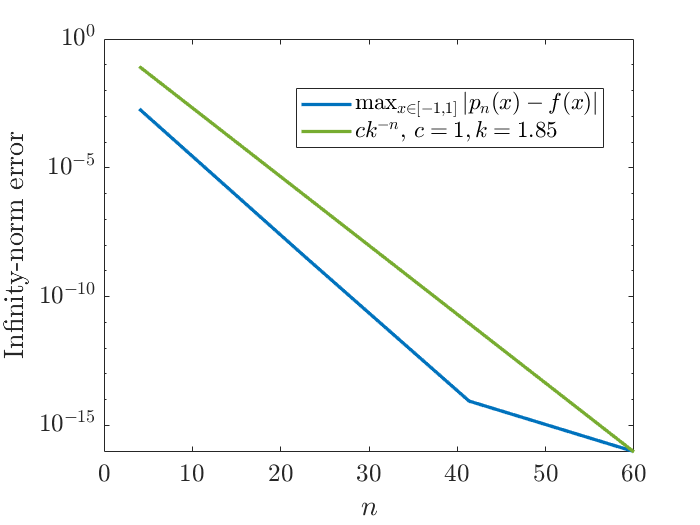
\includegraphics[scale=0.5]{graphics/plot-05-01.png}
    \caption{Infinity norm error of $f(x) = 1 / (25 x^2 + 1)$ and a bounding function}
  \end{figure}
\end{solution}

\begin{statement}{c}
  $f(x) = \cosh(\sin x)$.
\end{statement}

\begin{solution}
  Computing the infinity-norm error of $4001$ evenly spaced points between $-1$ and $1$
  of each polynomial interpolant, a good approximation for $k$ is $1.75$ using $c = 1$.
  \lstinputlisting{scripts/problems/problem-05-03.m}
  \begin{figure}[H]
    \centering
    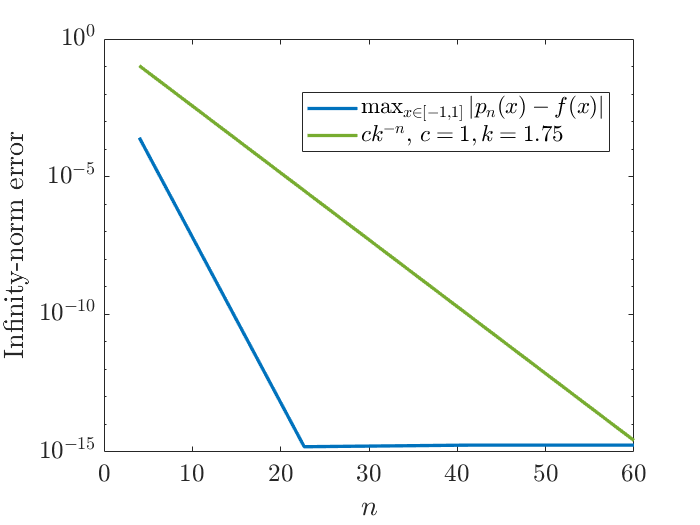
\includegraphics[scale=0.5]{graphics/plot-05-03.png}
    \caption{Infinite norm error of $f(x) = \cosh(\sin(x))$ and a bounding function}
  \end{figure}
\end{solution}

\end{document}
